\documentclass[%
a4paper,							% paper format
%landscape,						% Querformat
11pt,								% Schriftgröße (12pt, 11pt (Standard))
%BCOR1cm,							% Bindekorrektur, bspw. 1 cm
%DIVcalc,							% führt die Satzspiegelberechnung neu aus
%											  s. scrguide 2.4
%twoside,							% Doppelseiten
%twocolumn,						% zweispaltiger Satz
%halfparskip*,				% Absatzformatierung s. scrguide 3.1
%headsepline,					% Trennline zum Seitenkopf	
%footsepline,					% Trennline zum Seitenfuß
%titlepage,						% Titelei auf eigener Seite
%normalheadings,			% Überschriften etwas kleiner (smallheadings)
%idxtotoc,						% Index im Inhaltsverzeichnis
%listof=totoc,					% Abb.- und Tab.verzeichnis im Inhalt
bibliography=totoc,						% Literaturverzeichnis im Inhalt
abstracton,					% Überschrift über der Zusammenfassung an	
%leqno,   						% Nummerierung von Gleichungen links
%fleqn,								% Ausgabe von Gleichungen linksbündig
%draft								% überlangen Zeilen in Ausgabe gekennzeichnet
]
{scrartcl}

%%%%%%%%%%%%%%%%%%%%%%%%%%%%%%%%%%%%%%%%%%%%%%%%%%%%%%%%%%%%%%%%%%%%%%%%%%%%%%%%%%%%%%%%%%%%
%% Page Layout
%%%%%%%%%%%%%%%%%%%%%%%%%%%%%%%%%%%%%%%%%%%%%%%%%%%%%%%%%%%%%%%%%%%%%%%%%%%%%%%%%%%%%%%%%%%%
\usepackage[a4paper,left=3.0cm,right=2.5cm, top=2.5cm, bottom=3.0cm]{geometry}
\usepackage[headsepline=.4pt,footsepline=.4pt,automark,autooneside=false,]{scrlayer-scrpage}
\clearscrheadfoot 
\pagestyle{scrheadings} 
\automark[subsection]{section} 
\automark*[subsubsection]{subsection}
\ihead{\scriptsize\rightmark} 
\cfoot{\pagemark}
  
%%%%%%%%%%%%%%%%%%%%%%%%%%%%%%%%%%%%%%%%%%%%%%%%%%%%%%%%%%%%%%%%%%%%%%%%%%%%%%%%%%%%%%%%%%%%
%% language settings
%%%%%%%%%%%%%%%%%%%%%%%%%%%%%%%%%%%%%%%%%%%%%%%%%%%%%%%%%%%%%%%%%%%%%%%%%%%%%%%%%%%%%%%%%%%%
\usepackage[ngerman, english]{babel}
\usepackage[T1]{fontenc}
\usepackage[utf8]{inputenc}
\usepackage{lmodern}
\usepackage[onehalfspacing]{setspace} %1,5 spacing

%%%%%%%%%%%%%%%%%%%%%%%%%%%%%%%%%%%%%%%%%%%%%%%%%%%%%%%%%%%%%%%%%%%%%%%%%%%%%%%%%%%%%%%%%%%%
%% Spaces in commmands
%%%%%%%%%%%%%%%%%%%%%%%%%%%%%%%%%%%%%%%%%%%%%%%%%%%%%%%%%%%%%%%%%%%%%%%%%%%%%%%%%%%%%%%%%%%%
\usepackage{xspace}
%%%%%%%%%%%%%%%%%%%%%%%%%%%%%%%%%%%%%%%%%%%%%%%%%%%%%%%%%%%%%%%%%%%%%%%%%%%%%%%%%%%%%%%%%%%%
%% Internal LaTeX calculations
%%%%%%%%%%%%%%%%%%%%%%%%%%%%%%%%%%%%%%%%%%%%%%%%%%%%%%%%%%%%%%%%%%%%%%%%%%%%%%%%%%%%%%%%%%%%
\usepackage{calc}%\widthof{}

%%%%%%%%%%%%%%%%%%%%%%%%%%%%%%%%%%%%%%%%%%%%%%%%%%%%%%%%%%%%%%%%%%%%%%%%%%%%%%%%%%%%%%%%%%%%
%% Math-environments
%%%%%%%%%%%%%%%%%%%%%%%%%%%%%%%%%%%%%%%%%%%%%%%%%%%%%%%%%%%%%%%%%%%%%%%%%%%%%%%%%%%%%%%%%%%%
\usepackage{amsmath}
\usepackage{amssymb}
\usepackage{amsthm,thmtools}
\renewcommand\qedsymbol{$\square$}
\usepackage{mathtools}
\usepackage{ulsy}
\usepackage{bbm}
%problems with onehalfspacing
\begingroup
    \makeatletter
    \@for\theoremstyle:=definition,remark,plain\do{%
        \expandafter\g@addto@macro\csname th@\theoremstyle\endcsname{%
            \addtolength\thm@preskip\parskip
            }%
        }
\endgroup
\renewcommand{\theequation}{\thesection.\arabic{equation}}
\usepackage{chngcntr}%reset equation counter after each section
\counterwithin*{equation}{section}

\theoremstyle{plain}
\newtheorem{theorem}{Theorem}[section]
\newtheorem{lemma}[theorem]{Lemma}
\theoremstyle{definition}
\newtheorem{definition}[theorem]{Definition}
\newtheorem{assumption}[theorem]{Assumption}
\theoremstyle{remark}
\newtheorem{remark}[theorem]{Remark}
\theoremstyle{plain}
\newtheorem{proposition}[theorem]{Proposition}
\theoremstyle{plain}
\newtheorem{corollary}[theorem]{Corollary}
\theoremstyle{remark}
\newtheorem{example}[theorem]{Example}
%%%%%%%%%%%%%%%%%%%%%%%%%%%%%%%%%%%%%%%%%%%%%%%%%%%%%%%%%%%%%%%%%%%%%%%%%%%%%%%%%%%%%%%%%%%%
%% Table Packages
%%%%%%%%%%%%%%%%%%%%%%%%%%%%%%%%%%%%%%%%%%%%%%%%%%%%%%%%%%%%%%%%%%%%%%%%%%%%%%%%%%%%%%%%%%%%
\usepackage{tabularx}
% provides tabularx and X columns
\usepackage{booktabs}
% provides \toprule
\usepackage{multirow}
% provides \multirow
\usepackage{multicol}
% provides \multicol
\usepackage{pdflscape}

\usepackage{diagbox}
% provides \diagbox{bottom}{top}

% tables with pagebreak:
%\usepackage{tabu,longtable}
%\usepackage{ltxtable}%tabularx meets longtable
\usepackage{ltablex}%long_table_x
\keepXColumns

% reading external files into tables:
%\usepackage{pgfplotstable} % Generates table from .csv
%\pgfplotsset{compat=1.16}

% spacing adjustments:
\renewcommand{\arraystretch}{1.5}%1,5-facher Zeilenabstand in Tabellen
%%%%%%%%%%%%%%%%%%%%%%%%%%%%%%%%%%%%%%%%%%%%%%%%%%%%%%%%%%%%%%%%%%%%%%%%%%%%%%%%%%%%%%%%%%%%
%% List Packages
%%%%%%%%%%%%%%%%%%%%%%%%%%%%%%%%%%%%%%%%%%%%%%%%%%%%%%%%%%%%%%%%%%%%%%%%%%%%%%%%%%%%%%%%%%%%
\usepackage[flushleft]{paralist}
\setdefaultenum{(i)}{(a)}{(1)}{(aa)}%default numbering in law

%%%%%%%%%%%%%%%%%%%%%%%%%%%%%%%%%%%%%%%%%%%%%%%%%%%%%%%%%%%%%%%%%%%%%%%%%%%%%%%%%%%%%%%%%%%%
%% Color Packages
%%%%%%%%%%%%%%%%%%%%%%%%%%%%%%%%%%%%%%%%%%%%%%%%%%%%%%%%%%%%%%%%%%%%%%%%%%%%%%%%%%%%%%%%%%%%
\usepackage{color}
%\usepackage{xcolor}
%%%%%%%%%%%%%%%%%%%%%%%%%%%%%%%%%%%%%%%%%%%%%%%%%%%%%%%%%%%%%%%%%%%%%%%%%%%%%%%%%%%%%%%%%%%%
%% Verbatim Packages
%%%%%%%%%%%%%%%%%%%%%%%%%%%%%%%%%%%%%%%%%%%%%%%%%%%%%%%%%%%%%%%%%%%%%%%%%%%%%%%%%%%%%%%%%%%%
\usepackage{fancyvrb}
%%%%%%%%%%%%%%%%%%%%%%%%%%%%%%%%%%%%%%%%%%%%%%%%%%%%%%%%%%%%%%%%%%%%%%%%%%%%%%%%%%%%%%%%%%%%
%% Graphical Packages
%%%%%%%%%%%%%%%%%%%%%%%%%%%%%%%%%%%%%%%%%%%%%%%%%%%%%%%%%%%%%%%%%%%%%%%%%%%%%%%%%%%%%%%%%%%%
\usepackage{graphicx}
\usepackage{animate}
%\usepackage[allfiguresdraft]{draftfigure}
%\usepackage{svg}
\usepackage{tikz}
\usetikzlibrary{calc}
\usepackage{varwidth} 
% provides variable node width
\tikzset{
    max width/.style args={#1}{
        execute at begin node={\begin{varwidth}{#1}},
        execute at end node={\end{varwidth}}
    }
}
%%%%%%%%%%%%%%%%%%%%%%%%%%%%%%%%%%%%%%%%%%%%%%%%%%%%%%%%%%%%%%%%%%%%%%%%%%%%%%%%%%%%%%%%%%%%
%% TO DO & showkey Package
%%%%%%%%%%%%%%%%%%%%%%%%%%%%%%%%%%%%%%%%%%%%%%%%%%%%%%%%%%%%%%%%%%%%%%%%%%%%%%%%%%%%%%%%%%%%
\usepackage{todonotes}
% must be loaded after tikz
% provides \todo[]{}
\usepackage[notref,notcite]{showkeys}%notref for no section, %notcite for no bibtex
%\usepackage[final]{showkeys}
\renewcommand*\showkeyslabelformat[1]{%
  \fbox{\parbox[t]{.75\marginparwidth}{\raggedright\normalfont\tiny\ttfamily#1}}}
%%%%%%%%%%%%%%%%%%%%%%%%%%%%%%%%%%%%%%%%%%%%%%%%%%%%%%%%%%%%%%%%%%%%%%%%%%%%%%%%%%%%%%%%%%%%
%% Accents
%%%%%%%%%%%%%%%%%%%%%%%%%%%%%%%%%%%%%%%%%%%%%%%%%%%%%%%%%%%%%%%%%%%%%%%%%%%%%%%%%%%%%%%%%%%%
%\usepackage{accents}
%\newcommand{\ubar}[1]{\underaccent{\bar}{#1}}
%\newcommand{\ubar}[1]{\text{\b{$#1$}}}
%%%%%%%%%%%%%%%%%%%%%%%%%%%%%%%%%%%%%%%%%%%%%%%%%%%%%%%%%%%%%%%%%%%%%%%%%%%%%%%%%%%%%%%%%%%%
%% table of contents settings
%%%%%%%%%%%%%%%%%%%%%%%%%%%%%%%%%%%%%%%%%%%%%%%%%%%%%%%%%%%%%%%%%%%%%%%%%%%%%%%%%%%%%%%%%%%%
%\setcounter{secnumdepth}{6}
%\setcounter{tocdepth}{6}

%%%%%%%%%%%%%%%%%%%%%%%%%%%%%%%%%%%%%%%%%%%%%%%%%%%%%%%%%%%%%%%%%%%%%%%%%%%%%%%%%%%%%%%%%%%%
%% float object settings
%%%%%%%%%%%%%%%%%%%%%%%%%%%%%%%%%%%%%%%%%%%%%%%%%%%%%%%%%%%%%%%%%%%%%%%%%%%%%%%%%%%%%%%%%%%%
\usepackage{float}
%\setcounter{topnumber}{1}
%\setcounter{bottomnumber}{0}
%\setcounter{totalnumber}{1}
\usepackage{placeins}
%Defines a \FloatBarrier command, beyond which floats may not pass; useful, for example, to ensure all floats for a section appear before the next \section command.
%%%%%%%%%%%%%%%%%%%%%%%%%%%%%%%%%%%%%%%%%%%%%%%%%%%%%%%%%%%%%%%%%%%%%%%%%%%%%%%%%%%%%%%%%%%%
%% bibliography
%%%%%%%%%%%%%%%%%%%%%%%%%%%%%%%%%%%%%%%%%%%%%%%%%%%%%%%%%%%%%%%%%%%%%%%%%%%%%%%%%%%%%%%%%%%%
\usepackage{csquotes}
\usepackage[
	backend=bibtex,
	%backend=biber,
	style=bwl-FU,
	natbib=true,
	sortcites=true,
	block=space
]{biblatex}
\renewcommand*{\mkbibnamefamily}[1]{\textsc{#1}}
\renewcommand*{\mkbibnamegiven}[1]{\textsc{#1}}
\renewcommand*{\finalnamedelim}{\ \bibstring{and}\ }
%\renewcommand*{\finalnamedelim}{\textsc{ \bibstring{and} }}
%\addbibresource{literature.bib}

%%%%%%%%%%%%%%%%%%%%%%%%%%%%%%%%%%%%%%%%%%%%%%%%%%%%%%%%%%%%%%%%%%%%%%%%%%%%%%%%%%%%%%%%%%%%
%% Cross-Referencing
%%%%%%%%%%%%%%%%%%%%%%%%%%%%%%%%%%%%%%%%%%%%%%%%%%%%%%%%%%%%%%%%%%%%%%%%%%%%%%%%%%%%%%%%%%%%
\usepackage{titleref}
\usepackage{hyperref}
\usepackage{cleveref}
\hypersetup{
    colorlinks,
    %linkcolor={black},
		linkcolor={red},
    citecolor={blue},
    urlcolor={blue}
}
\begin{document}
\pagestyle{scrheadings}
%\input{Pdf/temp/exm.tex}
%%\IfFileExists{./filename}{true-branch}{false-branch}
%\IfFileExists{./Pdf/ComputerSpecifics/comp_spec.tex}{%
%\subsubsection*{Hardware}
%\input{Pdf/ComputerSpecifics/comp_spec.tex}
%}
\section{Rating transition model}
\subsection{Calibration Parameters}
	\newcommand{\calibrationParametersP}{
\begin{tabular}{*{4}{c}}
From-To & a & b & sigma\\
\toprule1-2 & 1.57e+00 & 4.69e-02 & 5.76e-02\\
1-3 & 1.62e+00 & 8.83e-03 & 1.15e-02\\
1-4 & 1.53e+00 & 2.05e-01 & 3.22e-02\\
2-1 & 1.54e+00 & 6.91e-02 & 9.68e-02\\
2-3 & 1.44e+00 & 3.14e-03 & 5.75e-03\\
2-4 & 1.46e+00 & 9.98e-02 & 9.50e-02\\
3-1 & 7.87e-01 & 1.42e-04 & 1.10e-04\\
3-2 & 5.76e-01 & 1.00e-04 & 1.00e-04\\
3-4 & 1.51e+00 & 6.42e-01 & 5.10e-02\end{tabular}
}
\newcommand{\calibrationParametersQ}{
$h=\left[21.763\ 15.131\ 31.669\ \right]$}

	\calibrationParametersP


	\calibrationParametersQ


\subsection{Computational Times}
	\newcommand{\ctimeCalP}{497.248}
\newcommand{\ctimeCalQ}{84.5601}
\newcommand{\compTimes}{
\begin{compactenum}
\item Calibration time under P using 301 points for the Euler scheme and 1000 trajectories: \ctimeCalP seconds.
\item Calibration time under Q using 301 points for the Euler scheme and 1000 trajectories: \ctimeCalQ seconds.
\end{compactenum}
}

	\compTimes


\subsection{Errors}
	\newcommand{\errorCalP}{2.04551e-07}
\newcommand{\errorCalQ}{0.00105951}
\newcommand{\errors}{
\begin{compactenum}
\item Calibration error under P using 301 points for the Euler scheme and 1000 trajectories: \errorCalP.
\item Calibration error under Q using 301 points for the Euler scheme and 1000 trajectories: \errorCalQ.
\end{compactenum}
}

	\errors


\subsection{Rating Properties}
\paragraph*{TimeGAN}
	\newcommand{\mDCRec}{
Monotone default column\\
\begin{tabular}{*{5}{c}}
  & t=0.083 & t=0.25 & t=0.5 & t=1\\
\toprule1-2 & 1 & 1 & 1 & 1\\
2-3 & 1 & 1 & 1 & 1\\
3-4 & 1 & 1 & 1 & 1\end{tabular}
}
\newcommand{\sDDRec}{
Strongly diagonal dominant\\
\begin{tabular}{*{5}{c}}
  & t=0.083 & t=0.25 & t=0.5 & t=1\\
\toprule1 & 1 & 1 & 1 & 1\\
2 & 1 & 1 & 1 & 1\\
3 & 1 & 1 & 1 & 1\\
4 & 1 & 1 & 1 & 1\end{tabular}
}
\newcommand{\dMLRec}{
Down more likely\\
\begin{tabular}{*{5}{c}}
t=0.083 & t=0.25 & t=0.5 & t=1\\
\toprule1 & 1 & 1 & 1\end{tabular}
}
\newcommand{\iRSRec}{
Increasing rating spread\\
\begin{tabular}{*{4}{c}}
  & dt=0.25-0.083 & dt=0.5-0.25 & dt=1-0.5\\
\toprule1 & 1 & 1 & 1\\
2 & 1 & 1 & 1\\
3 & 1 & 1 & 1\\
4 & 1 & 1 & 1\end{tabular}
}
\newcommand{\rSORec}{
Row sum one\\
\begin{tabular}{*{5}{c}}
  & t=0.083 & t=0.25 & t=0.5 & t=1\\
\toprule1 & 1.00e+00 & 1.00e+00 & 1.00e+00 & 1.00e+00\\
2 & 1.00e+00 & 1.00e+00 & 1.00e+00 & 1.00e+00\\
3 & 1.00e+00 & 1.00e+00 & 1.00e+00 & 1.00e+00\\
4 & 1 & 1 & 1 & 1\end{tabular}
}

	\mDCRec


	\sDDRec


	\dMLRec


	\iRSRec


	\rSORec


\paragraph*{SDE under P}
	\newcommand{\mDCSDEP}{
Monotone default column\\
\begin{tabular}{*{5}{c}}
  & t=0.083 & t=0.25 & t=0.5 & t=1\\
\toprule1-2 & 1 & 1 & 1 & 1\\
2-3 & 9.63e-01 & 1 & 1 & 1\\
3-4 & 1 & 1 & 1 & 1\end{tabular}
}
\newcommand{\sDDSDEP}{
Strongly diagonal dominant\\
\begin{tabular}{*{5}{c}}
  & t=0.083 & t=0.25 & t=0.5 & t=1\\
\toprule1 & 1 & 1 & 1 & 1\\
2 & 1 & 1 & 1 & 1\\
3 & 1 & 1 & 1 & 1\\
4 & 1 & 1 & 1 & 1\end{tabular}
}
\newcommand{\dMLSDEP}{
Down more likely\\
\begin{tabular}{*{5}{c}}
t=0.083 & t=0.25 & t=0.5 & t=1\\
\toprule9.78e-01 & 9.97e-01 & 1 & 1\end{tabular}
}
\newcommand{\iRSSDEP}{
Increasing rating spread\\
\begin{tabular}{*{4}{c}}
  & dt=0.25-0.083 & dt=0.5-0.25 & dt=1-0.5\\
\toprule1 & 1 & 1 & 1\\
2 & 1 & 1 & 1\\
3 & 1 & 1 & 1\\
4 & 1 & 1 & 1\end{tabular}
}
\newcommand{\rSOSDEP}{
Row sum one\\
\begin{tabular}{*{5}{c}}
  & t=0.083 & t=0.25 & t=0.5 & t=1\\
\toprule1 & 1 & 1 & 1 & 1\\
2 & 1 & 1 & 1 & 1\\
3 & 1 & 1 & 1 & 1\\
4 & 1 & 1 & 1 & 1\end{tabular}
}

	\mDCSDEP


	\sDDSDEP


	\dMLSDEP


	\iRSSDEP


	\rSOSDEP


\paragraph*{SDE under Q}
	\newcommand{\mDCSDEQ}{
Monotone default column\\
\begin{tabular}{*{5}{c}}
  & t=0.083 & t=0.25 & t=0.5 & t=1\\
\toprule1-2 & 1 & 1 & 1 & 1\\
2-3 & 9.75e-01 & 1 & 1 & 1\\
3-4 & 1 & 1 & 1 & 1\end{tabular}
}
\newcommand{\sDDSDEQ}{
Strongly diagonal dominant\\
\begin{tabular}{*{5}{c}}
  & t=0.083 & t=0.25 & t=0.5 & t=1\\
\toprule1 & 1 & 1 & 1 & 1\\
2 & 1 & 1 & 1 & 1\\
3 & 1 & 1 & 1 & 1\\
4 & 1 & 1 & 1 & 1\end{tabular}
}
\newcommand{\dMLSDEQ}{
Down more likely\\
\begin{tabular}{*{5}{c}}
t=0.083 & t=0.25 & t=0.5 & t=1\\
\toprule9.76e-01 & 9.96e-01 & 1 & 1\end{tabular}
}
\newcommand{\iRSSDEQ}{
Increasing rating spread\\
\begin{tabular}{*{4}{c}}
  & dt=0.25-0.083 & dt=0.5-0.25 & dt=1-0.5\\
\toprule1 & 1 & 1 & 1\\
2 & 1 & 1 & 1\\
3 & 1 & 1 & 1\\
4 & 1 & 1 & 1\end{tabular}
}
\newcommand{\rSOSDEQ}{
Row sum one\\
\begin{tabular}{*{5}{c}}
  & t=0.083 & t=0.25 & t=0.5 & t=1\\
\toprule1 & 1 & 1 & 1 & 1\\
2 & 1 & 1 & 1 & 1\\
3 & 1 & 1 & 1 & 1\\
4 & 1 & 1 & 1 & 1\end{tabular}
}

	\mDCSDEQ


	\sDDSDEQ


	\dMLSDEQ


	\iRSSDEQ


	\rSOSDEQ


\subsection{Plots of Distributions}
	\begin{minipage}[c][][c]{\linewidth}
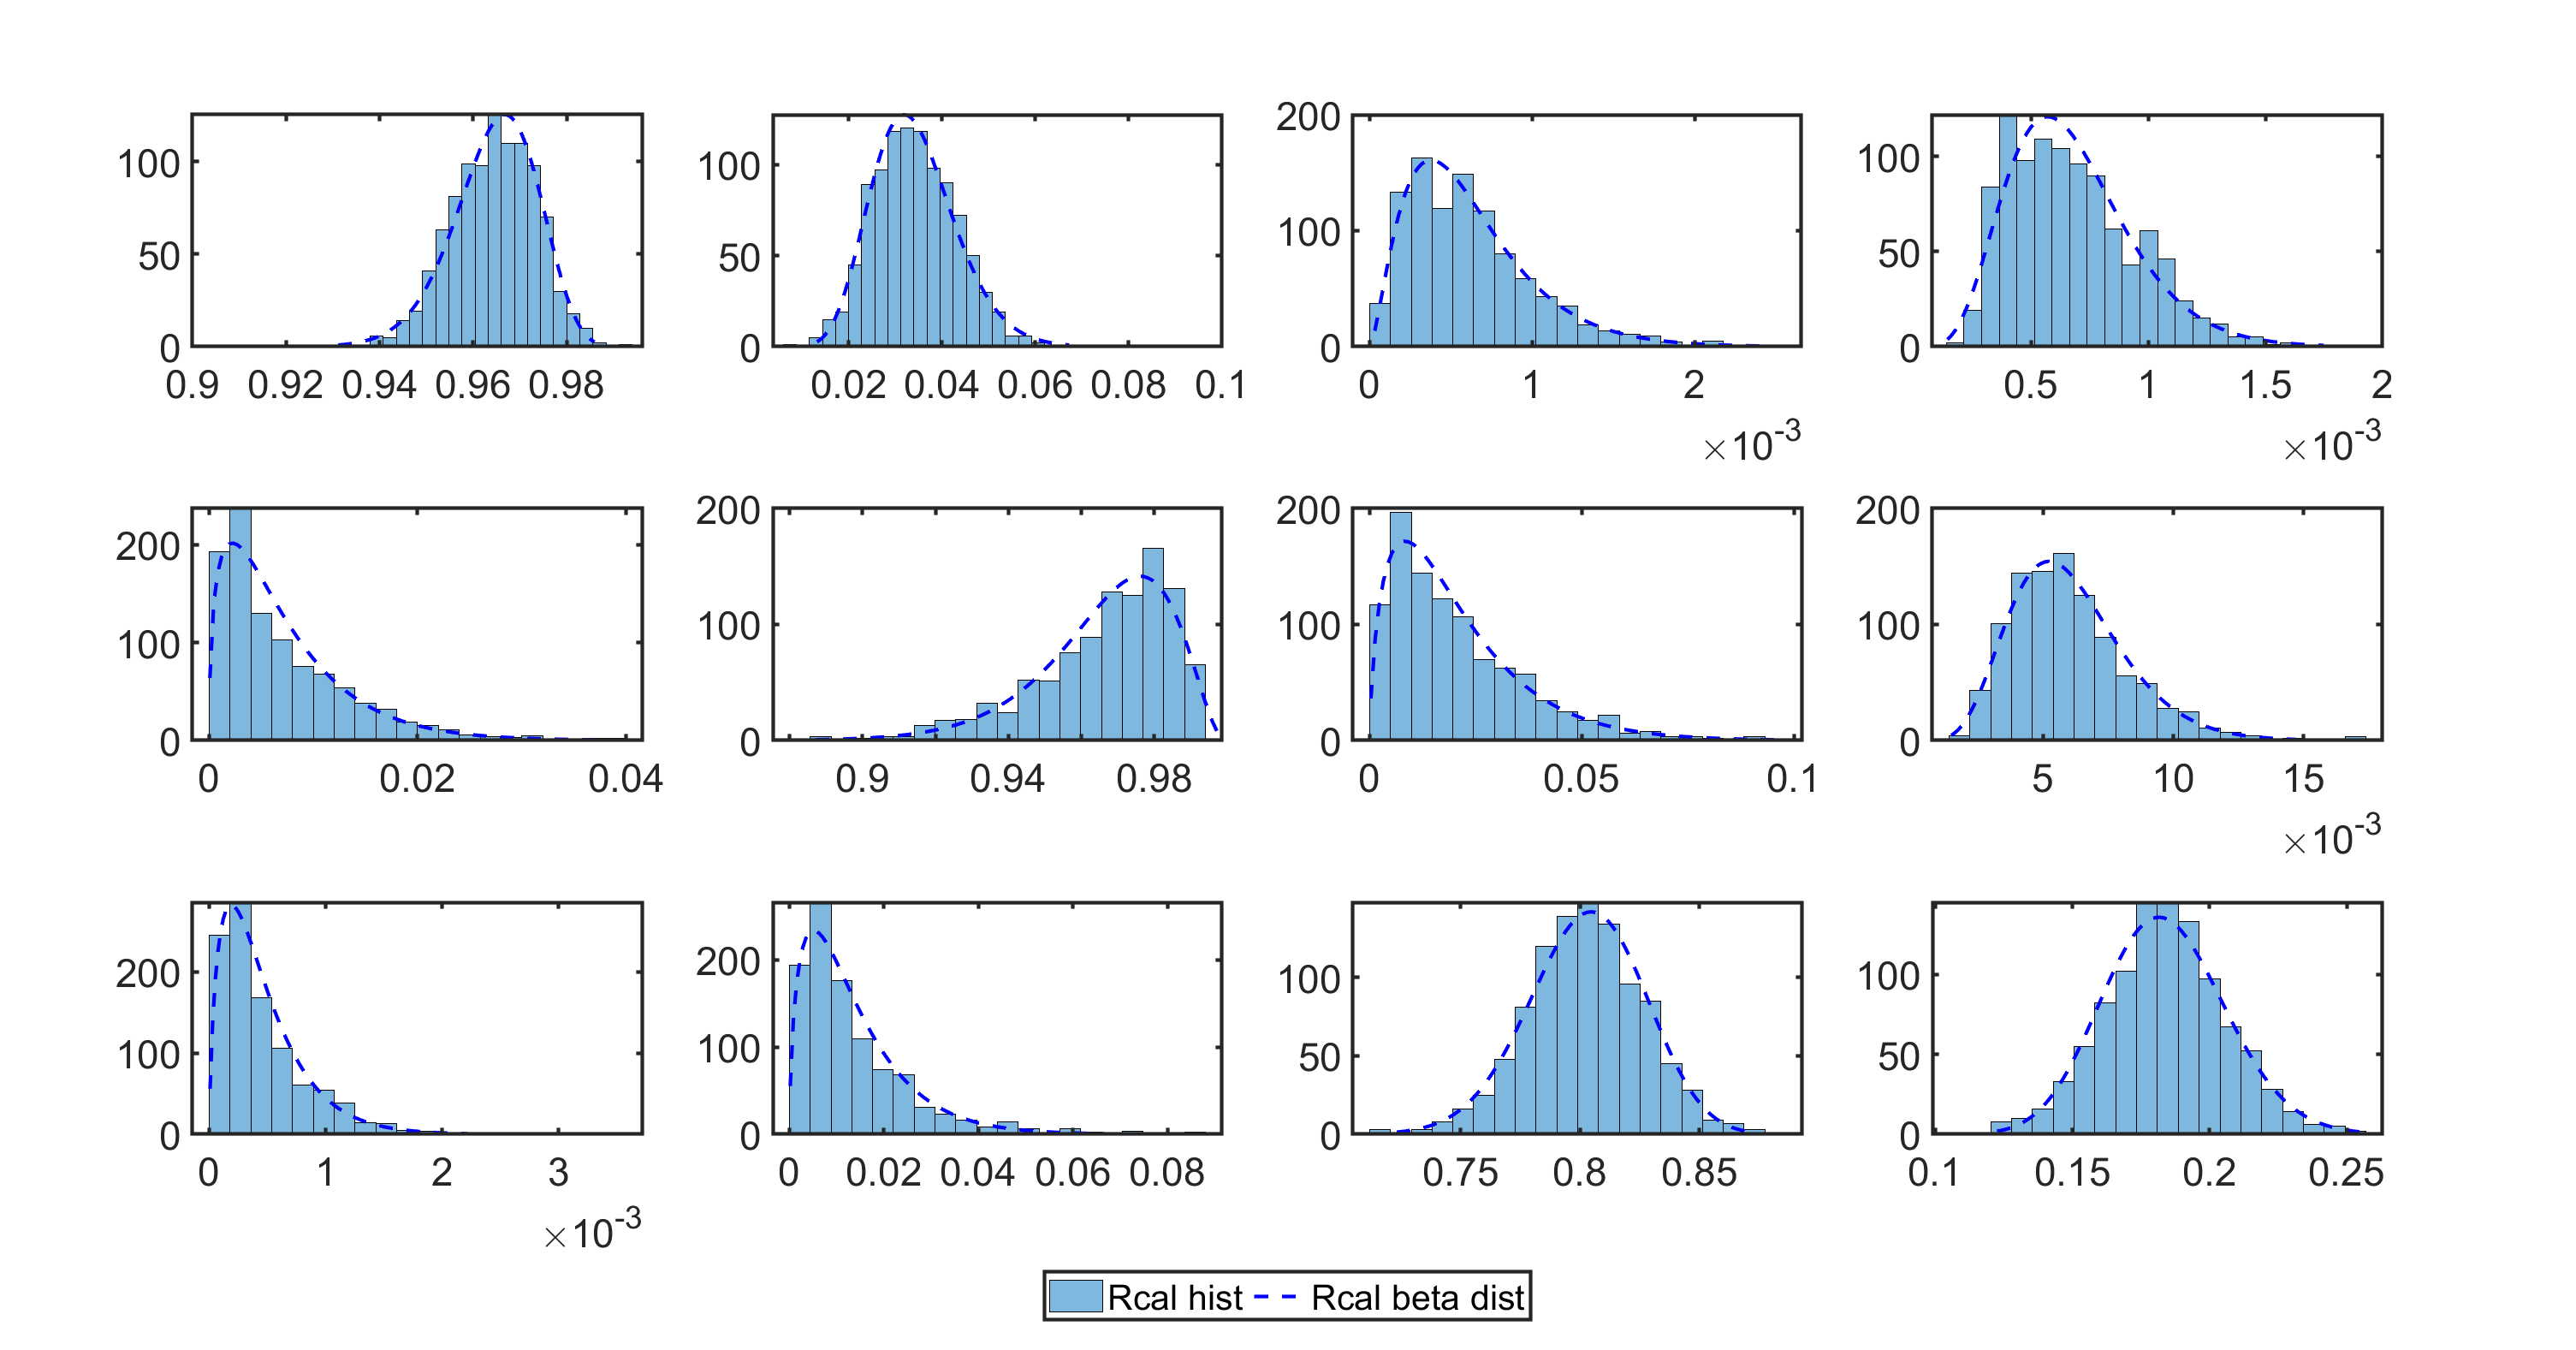
\includegraphics[width=.95\columnwidth]{RD_P/RD_P_1}
\end{minipage}

\subsection{Plots of Distributions}
	\begin{minipage}[c][][c]{\linewidth}
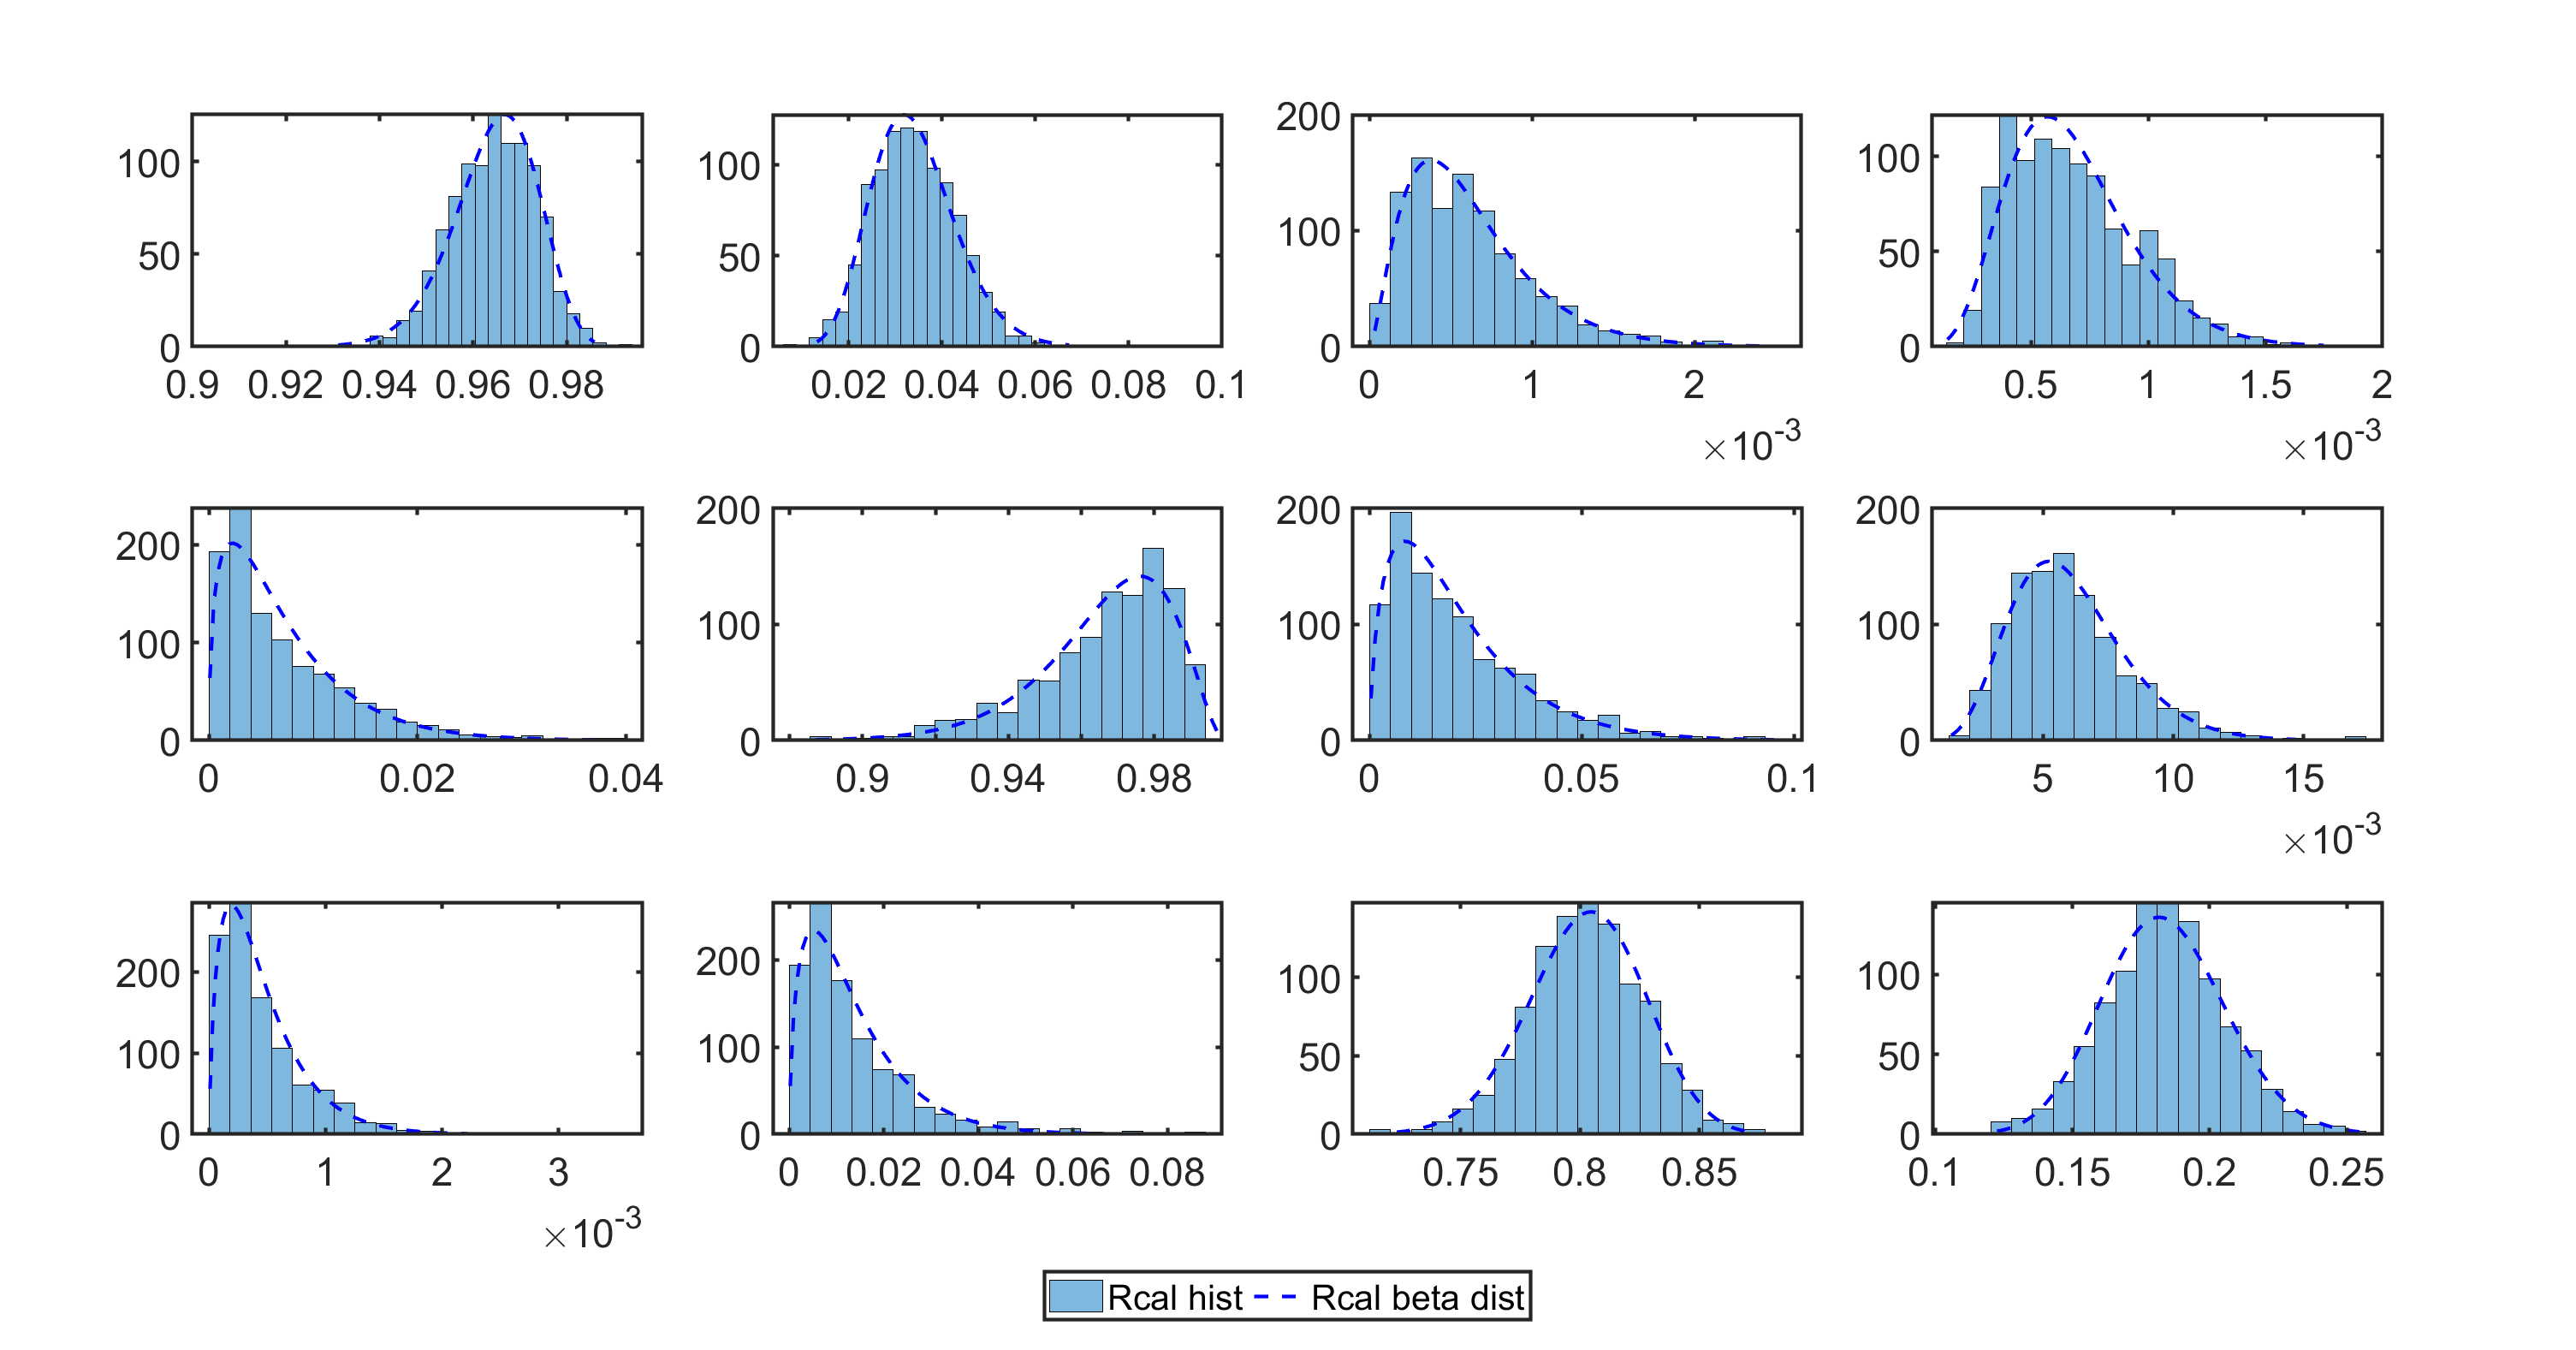
\includegraphics[width=.95\columnwidth]{RD_P/RD_P_1}
\end{minipage}

\subsection{Plots of Trajectories}
	\begin{minipage}[c][][c]{\linewidth}
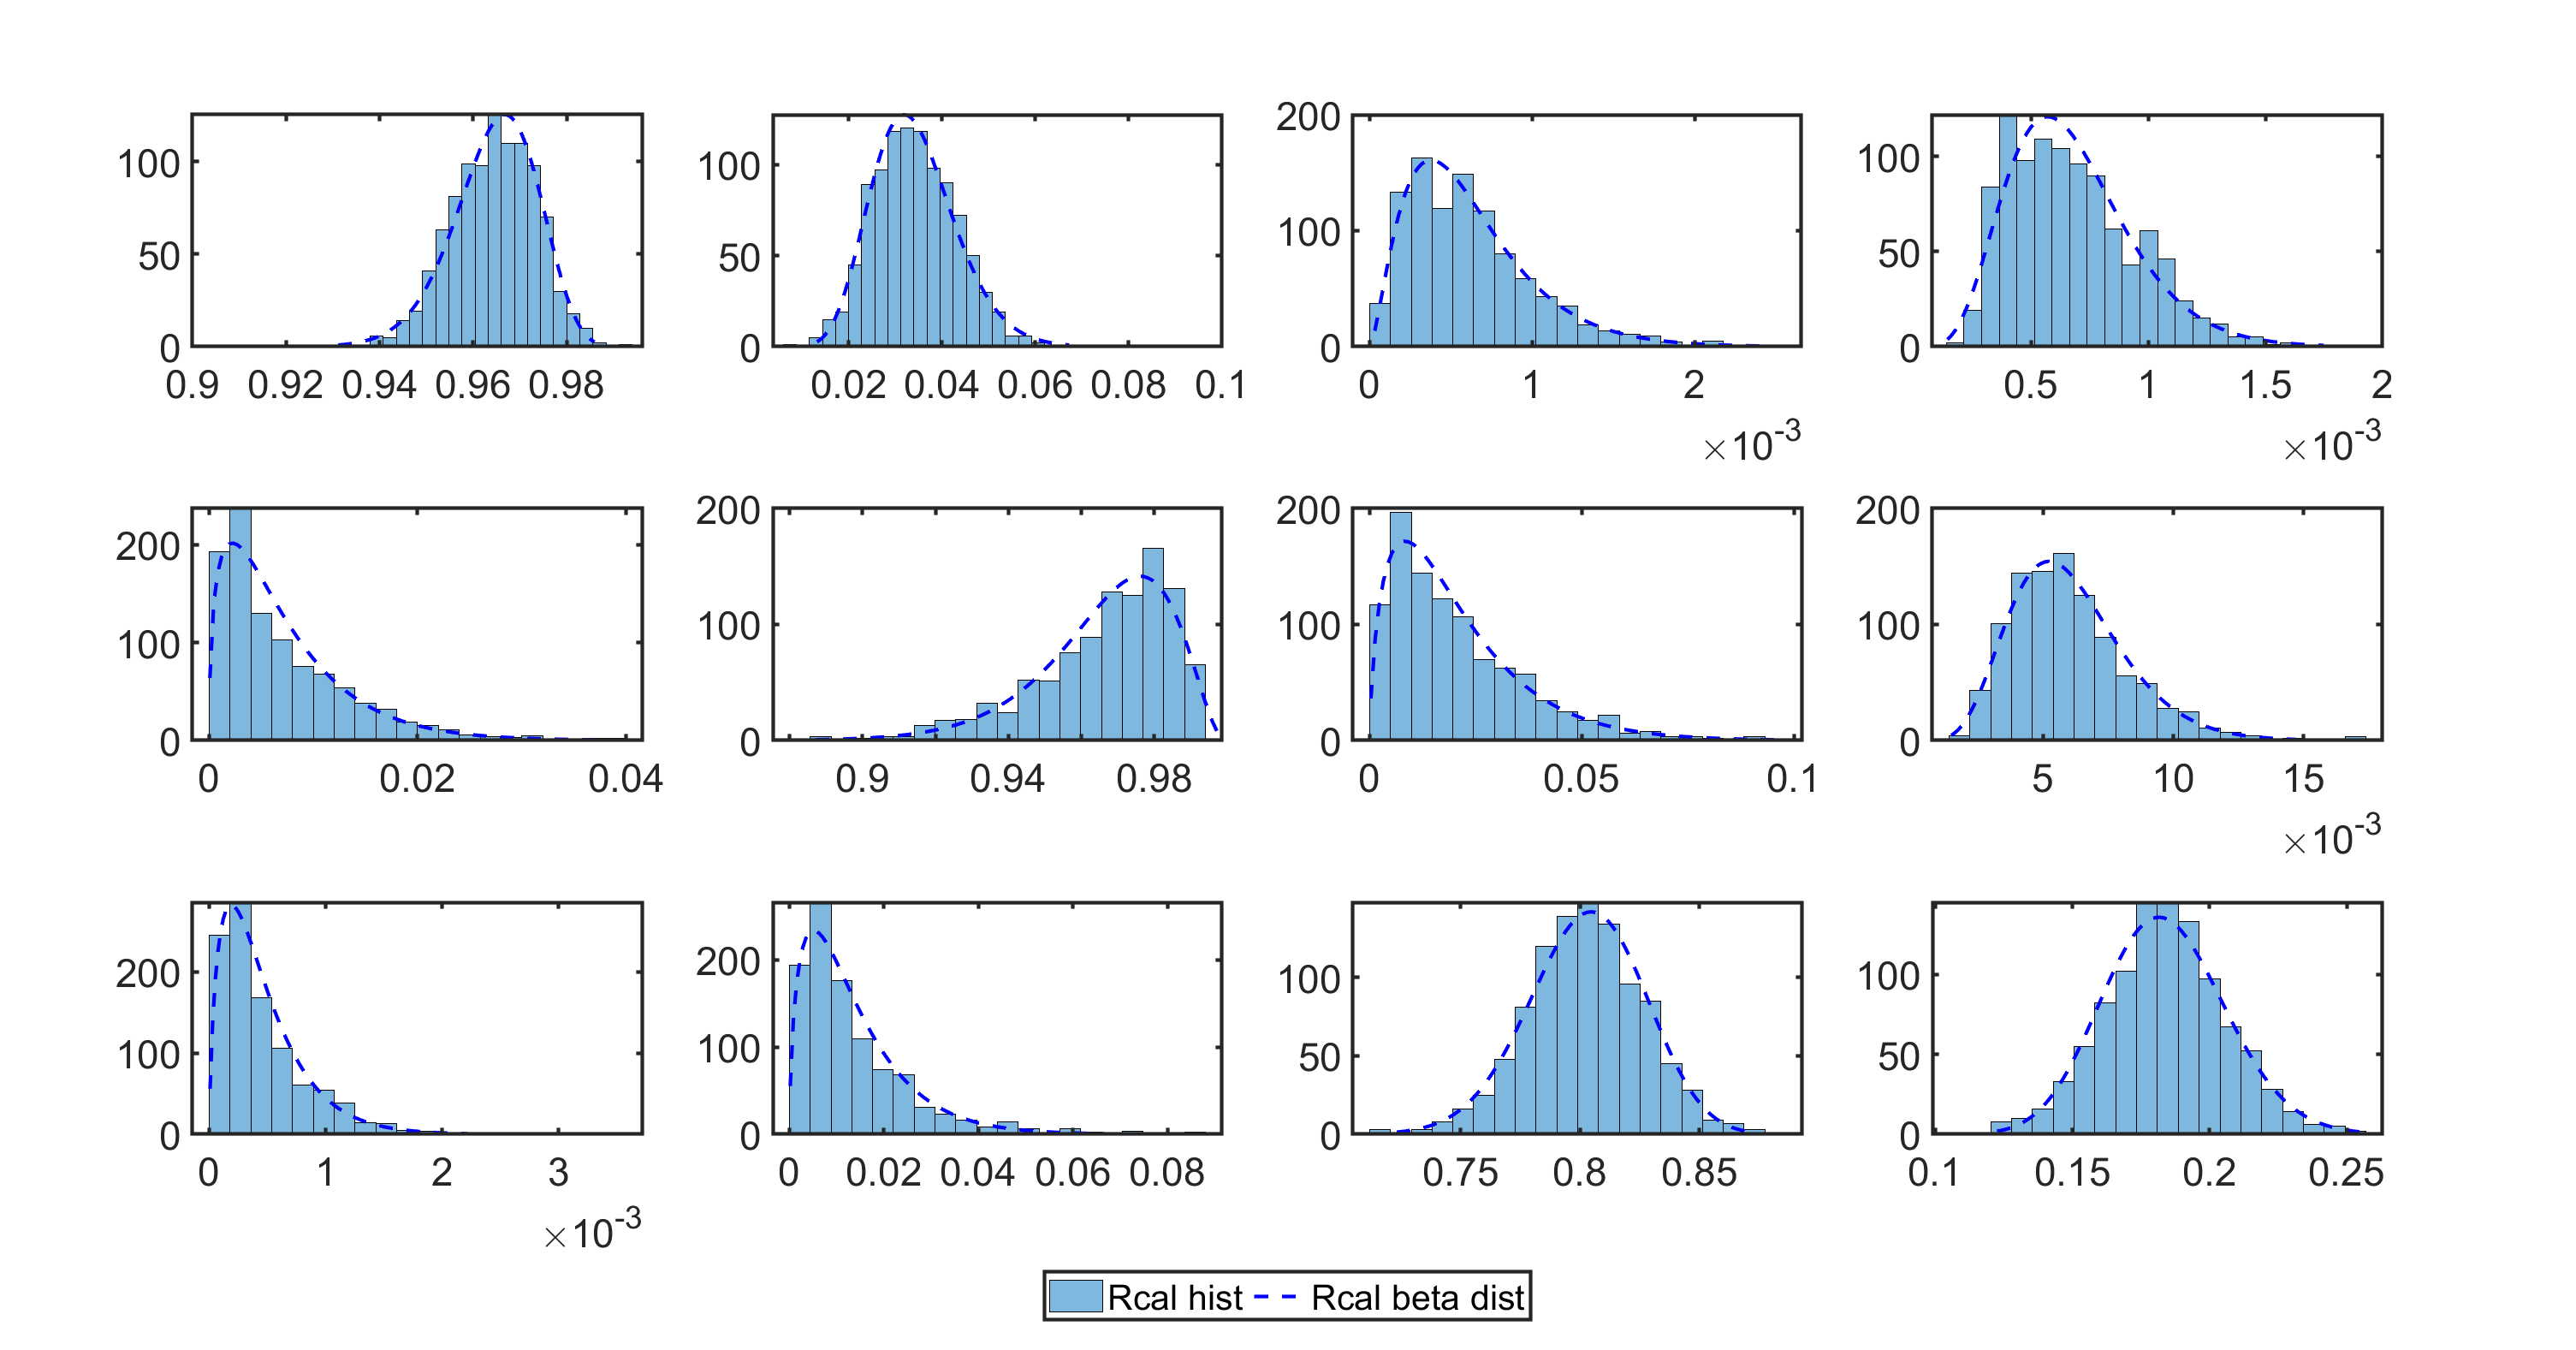
\includegraphics[width=.95\columnwidth]{RD_P/RD_P_1}
\end{minipage}

\subsection{Plots of Trajectories}
	\begin{minipage}[c][][c]{\linewidth}
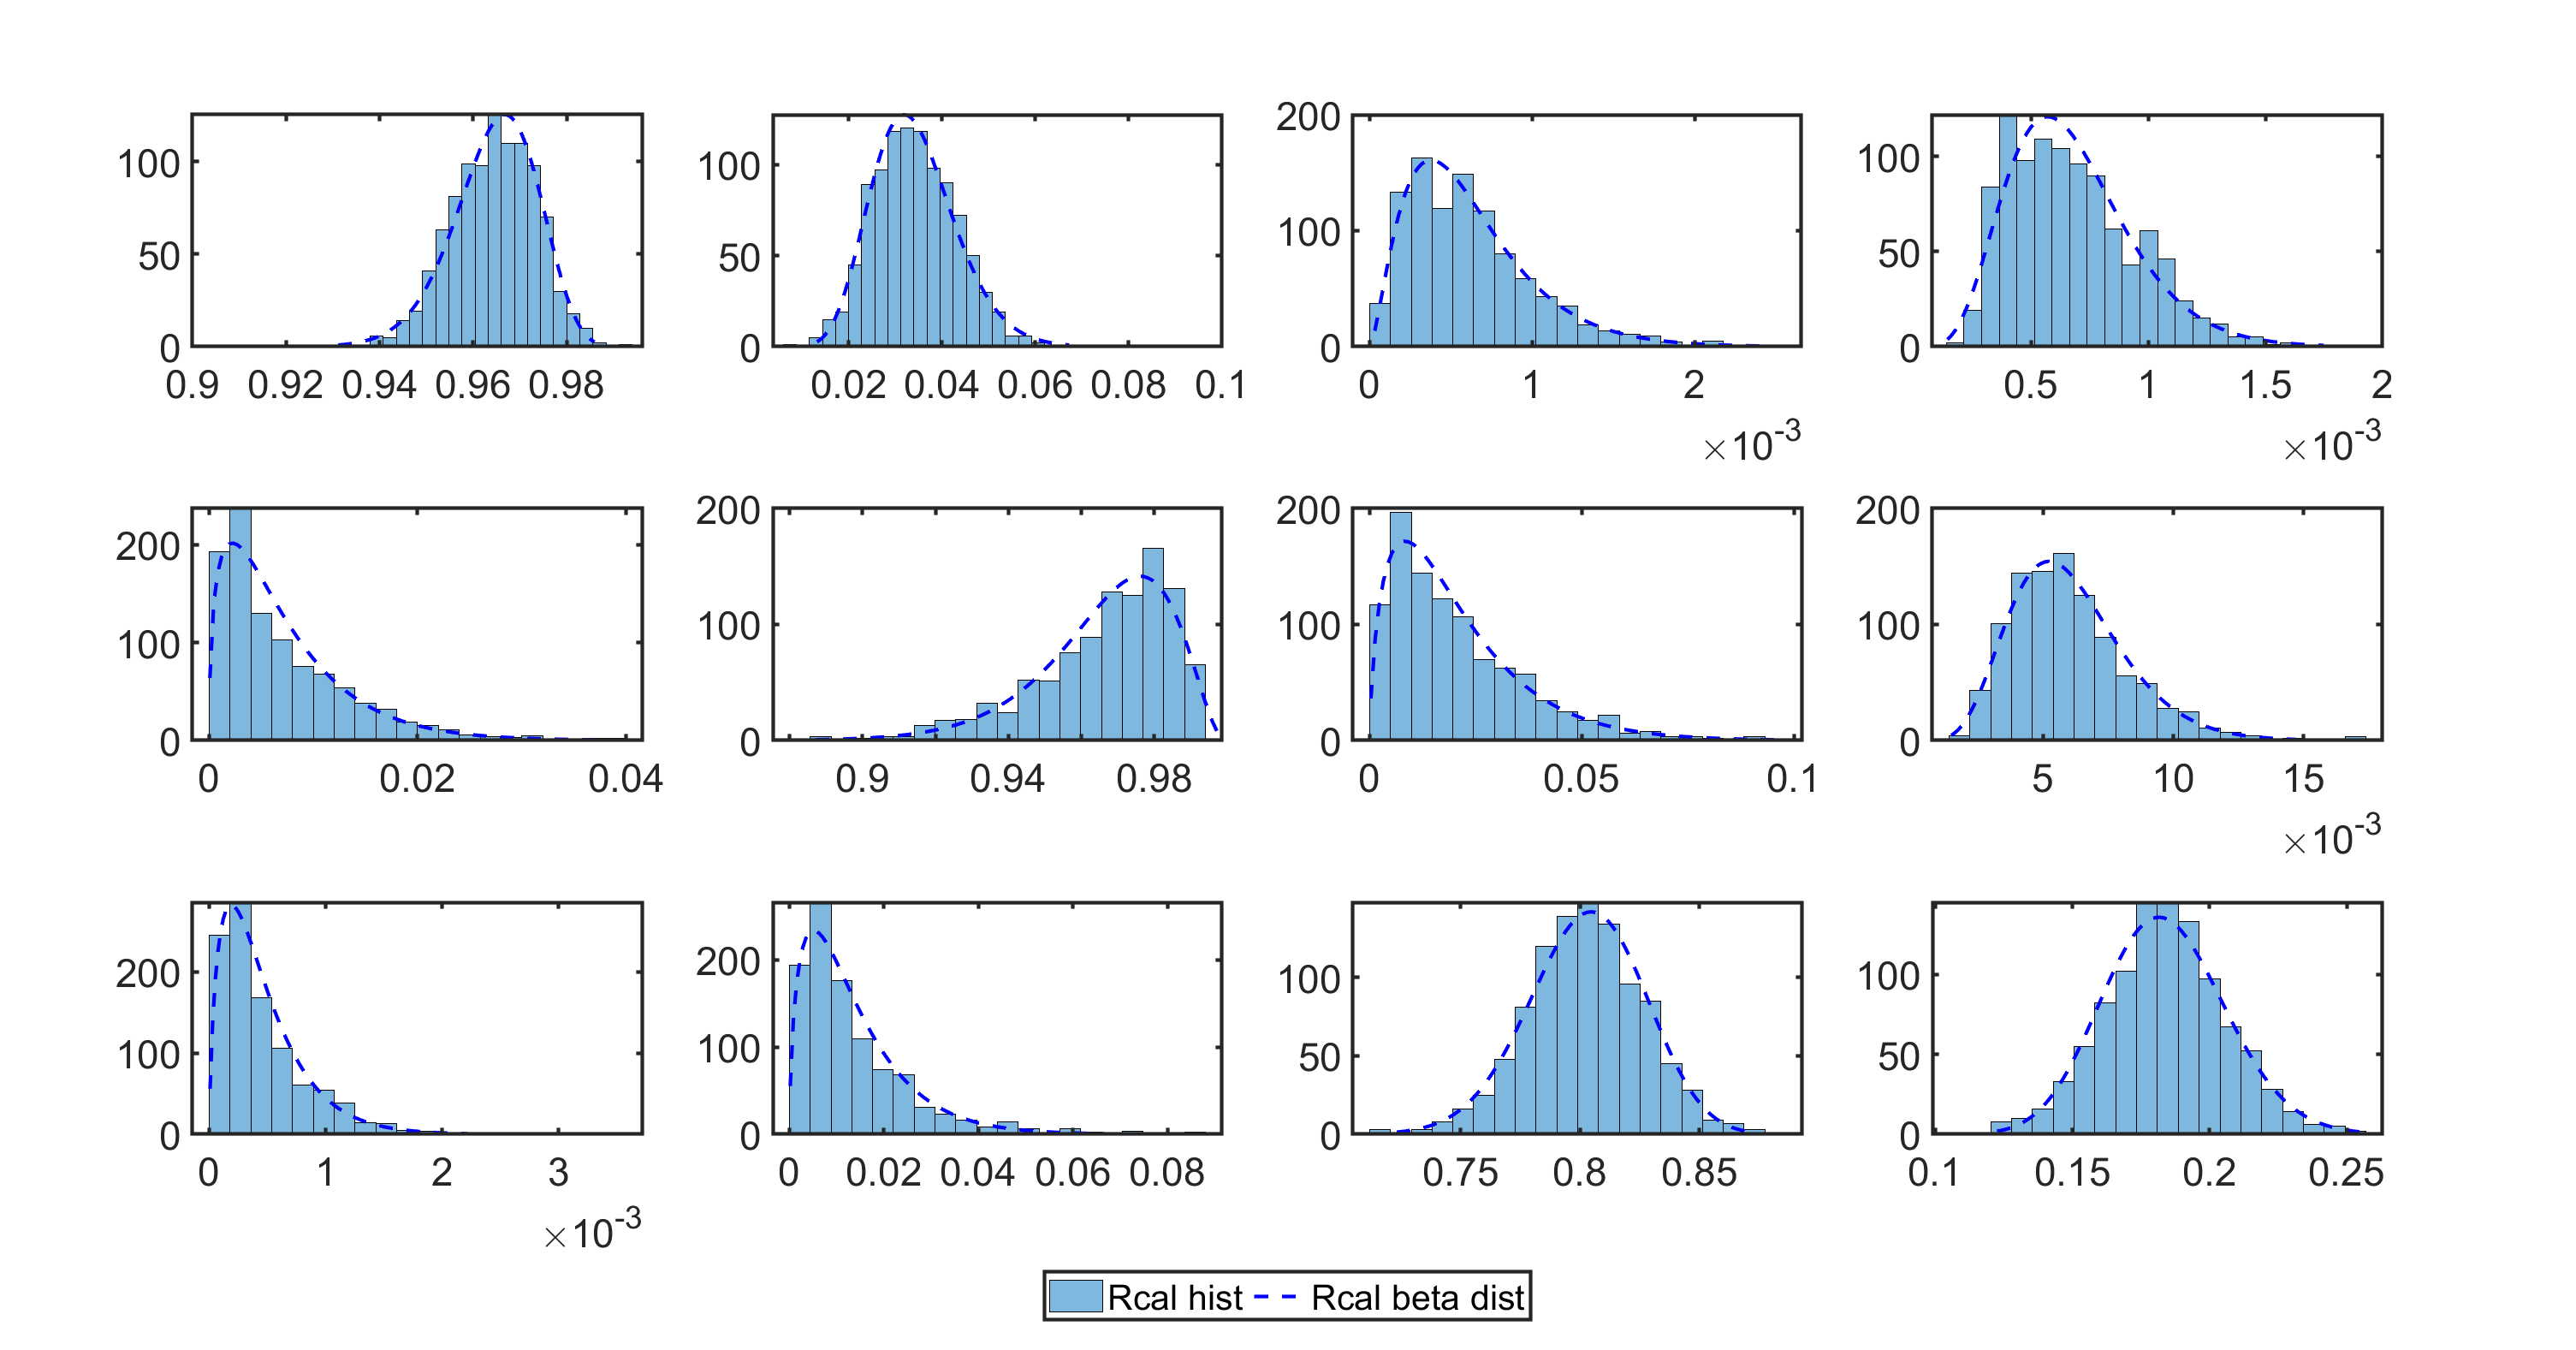
\includegraphics[width=.95\columnwidth]{RD_P/RD_P_1}
\end{minipage}


%\subsubsection*{Parameters}
	%%\begin{table}%
		%\input{Pdf/temp/param.tex}
		%%\caption{}
		%%\label{}
	%%\end{table}
%\subsubsection*{Errors}
	%%\begin{table}%
		%\newcommand{\errorCalP}{2.04551e-07}
\newcommand{\errorCalQ}{0.00105951}
\newcommand{\errors}{
\begin{compactenum}
\item Calibration error under P using 301 points for the Euler scheme and 1000 trajectories: \errorCalP.
\item Calibration error under Q using 301 points for the Euler scheme and 1000 trajectories: \errorCalQ.
\end{compactenum}
}

		%%\caption{}
		%%\label{}
	%%\end{table}
%\subsubsection*{Computational times}
	%%\begin{table}%
		%\input{Pdf/temp/ctimes.tex}
		%%\caption{}
		%%\label{}
	%%\end{table}
%\subsubsection*{Figures}
		%\input{Pdf/temp/figures.tex}
%%\begin{landscape}
	%%%\begin{figure}%
	%%\includegraphics[width=.95\columnwidth]{Pdf/temp/figures.png}%
	%%%\caption{}%
	%%%\label{}%
	%%%\end{figure}
%%\end{landscape}
\end{document}